\section{Praktische Teilumsetzung des Konzepts 3.0 an ausgewählten Versuchsständen}

Gemäß der Aufgabenstellung wurde zu Beginn des Projekts eine Analyse durchgeführt, um herauszufinden wie viele Versuchsstände digitale Schnittstellen besitzen. In Folge dessen wurde der \textit{Grad der Digitalisierung} definiert (Schnittstellen vorhanden, \glqq effektive\grqq{} Schnittstelle; gemäß Tabelle \ref{tab:grad_der_digitalisierung}) und ermittelt, wie hoch der prozentuale Anteil der MVT Versuchsstände ist, bei denen bereits Daten akquiriert werden können. Unter anderem war ein Ergebnis der Analyse, dass zwei Versuchsstände (Wirbelschicht und Filterkuchen), mit digitaler Messtechnik bzw. Sensoren aufgerüstet werden sollen. In den folgenden Abschnitten wird die praktische Modifikation der Versuchsstände erläutert.\\

\subsection{Filterkuchenversuchsanlage}

Im Rahmen dieser Arbeit wurde die Filterkuchenversuchsanlage (siehe Abbildung \ref{fig:filterkuchenversuchsstand})  aufgerüstet. Das Fließschema der Anlage zu Projektbeginn ist der Abbildung \ref{fig:schema_filterkuchenversuchsstand}
zu entnehmen. Bei diesem Versuchsstand gibt es zwei Absperrhähne. Der erste Absperrhahn ({\Hypatia H1}) verriegelt das Leitungssystem gegen die Vacuumpumpe ({\Hypatia A}), somit kann ein Unterdruck während Versuchsvorbereitungen oder umbauten aufgebaut werden. Das Manometer ({\Hypatia B}) ist in der Vacuumpumpe integriert. Der zweite Absperrhahn ({\Hypatia H2}) verriegelt den Trübebehälter ({\Hypatia J}), indem ein Rührer ({\Hypatia K}) das Aussedimentieren der Suspension unterbindet. Unter dem Trübebehälterbefinden sich Kuststoffklemmen ({\Hypatia G}) und Gummiringe , um die Filternutschen ({\Hypatia I}) zu fixieren und abzudichten. Die Filternutschen werden mit dem Filtratauffangbehälter ({\Hypatia D}) verbunden, welcher sich bei Versuchsstillstand auf einer Schutzplatte ({\Hypatia E}) befindet, um die Digitalwaage ({\Hypatia F}) vor einer Dauerlast zu bewahren. Des Weiteren schützt die Schutzplatte die Waage bei Versuchsumbauten. Vor dem Starten eines Versuchsdurchlaufs ist die Schutzplatte ({\Hypatia E}) zu entfernen und der Filtratauffangbehälter ({\Hypatia D}) auf der Waage zu positionieren. Zwischen der Vacuumpumpe (Richtung {\Hypatia A}) und dem Filtratauffangbehälter ({\Hypatia D}) befindet sich ein Pufferbehälter, um dem Pufferbehälter vor einer potentiellen Suspensionskontamination zu bewahren. Die Filterkuchenversuchsanlage wird im Rahmen der Präsenzveranstaltungen isobar betrieben. Die Gleichungen zur Berechnung der Filtrationsanlage sind dem Abschnitt \ref{sec:darcygleichung} zu entnehmen. Die linearisierte Filtrationsgleichung, auf der Grundlage der Darcy-Gleichung, ist nachfolgend aufgeführt:

\begin{equation}
\label{eq:irr_alpha_beta_kappa_integration_linearisiert_dpdt_2}
\frac{t}{V(t)} = \underbrace{\frac{\eta \cdot\alpha_\mathrm{V} \cdot \kappa}{A^2 \cdot 2 \cdot \Delta p_{\mathrm{konst,irr}}}
\cdot V(t)}_{\substack{a_1}}  +  \underbrace{\frac{\eta \cdot \beta}{A \cdot \Delta p_{\mathrm{konst,irr}}}}_{\substack{a_0}}
\end{equation}

Die zu bestimmenden Parameter sind der folgenden Auflistung zu entnehmen:

\begin{figure}[b!] % 
% \captionsetup{position=top}
    \centering
        \subfloat[][Filterkuchenversuchsstand vor den Modifikationen\label{fig:filterkuchenversuchsstand}]{%
            \hspace{0em}
            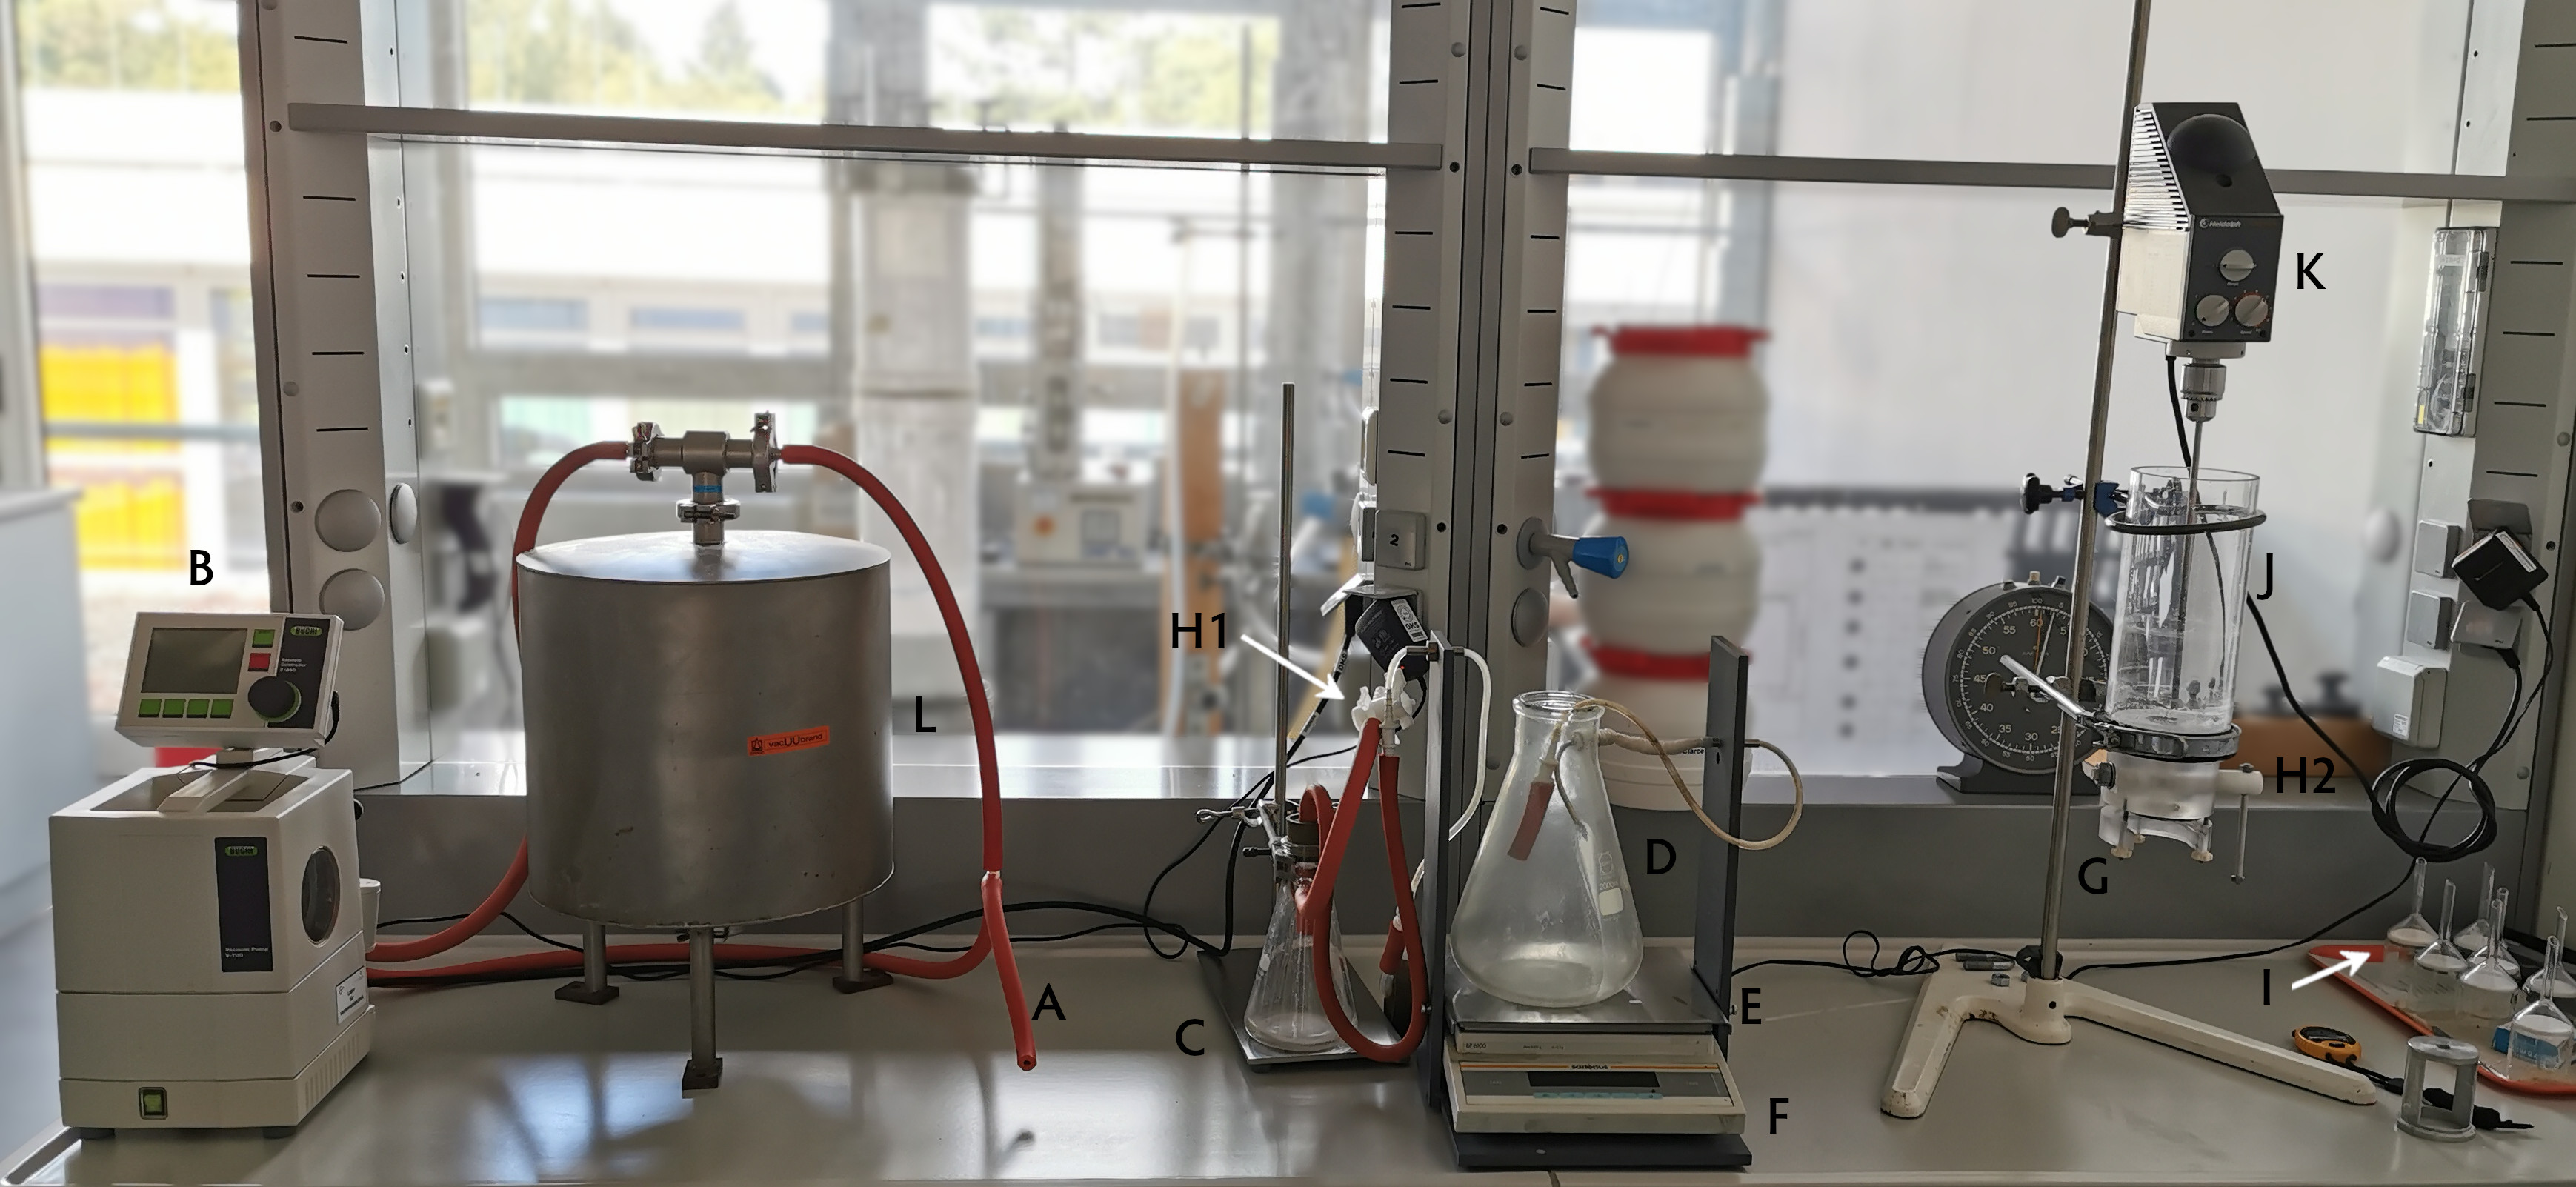
\includegraphics[width=1\textwidth]
            {Bilder/filterkuchversuchsstand.jpg} %{Bilder/LabVIEW_serialport/}
        }
    \phantomcaption
    \vspace{1em}
    \ContinuedFloat
%\captionsetup{position=bottom}
    \subfloat[Fließschema in Form einer schematischen Skizze der Filterkuchenversuchsanlage vor den Modifikationen]
    [Fließschema in Form einer schematischen Skizze der Filterkuchenversuchsanlage vor den Modifikationen \cite{Kuchenfiltration_Geweke2020} \label{fig:schema_filterkuchenversuchsstand}]{%
        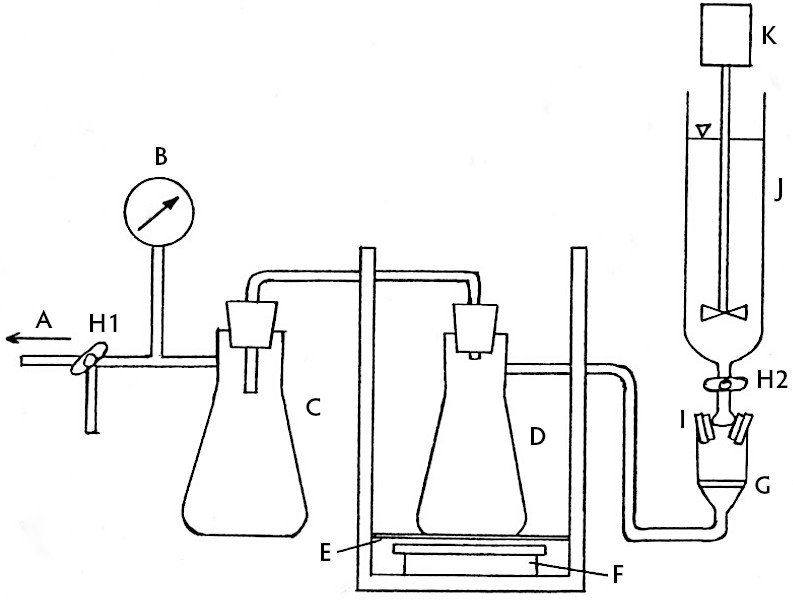
\includegraphics[width=0.75\textwidth]
        {Bilder/filterkuchversuch_schema.jpg} %{Bilder/LabVIEW_serialport/}
    }
    \caption[Filterkuchenversuchsanlage nach den Modifikationen]{Filterkuchenversuchsanlage nach den Modifikationen}
    \label{}
\end{figure}



\begin{enumerate}[label = \textbullet, itemsep = -.1em]
\item \textbf{diskret}
	\begin{enumerate}[label = --, itemsep = -.1em]
	\item a0
			\begin{enumerate}[label = -, itemsep = -.1em]
			\item die Viskosität $\eta$
			\item der Filtermittelwiderstand $\beta$
			\item die Filtrationsfläche $A$
			\end{enumerate}
	\item a1
		\begin{enumerate}[label = -, itemsep = -.1em]
		\item der Filterkuchenwiderstand $\alpha_\mathrm{V}$
		\item die Proportionalitätskonstante $\kappa$
		\item die Filtrationsfläche $A$
		\item die Viskosität $\eta$
		\end{enumerate}
	\item die Fluiddichte $\rho_\mathrm{f}$
	\item die Feststoffdichte $\rho_\mathrm{fs}$
	\end{enumerate}
	
\item \textbf{kontinuierlich}
	\begin{enumerate}[label = --, itemsep = -.1em]
	\item der irreversible Druckverlust $\Delta p_{\mathrm{konst,irr}}$
	\item das Volumen als Funktion der Zeit $V(t)=$\,\text{\Large{$\frac{m_{\mathrm{Filtrat}}(t)}{{\Large \rho_\mathrm{f}}}$}}
	\end{enumerate}

\end{enumerate}

Das Filtrationsvolumen, als Funktion der Zeit, wird über die zusammengesetzte, extensive Zustandsgröße -- der Filtratmasse $m_{\mathrm{Filtrat}}(t)$ -- bestimmt. 

\subsubsection{Sensorauswahl}

  

Im Betrieb der Filterkuchenversuchsanlage sind die Parameter, Volumenstrom $\dot{V}$ und Druck $p$, kontinuierlich zu erfassen. Die Masse des Filtrats wird von einer Laborwaage des Unternehmens Sartorius AG des Typs Practum 5101-1S detektiert. Die Waage hat eine USB Schnittstelle, die mit einem USB Kabel eine RS-232 Schnittstelle emuliert. Dafür sind, gemäß der Bedienungsanweisung der Waage, die Einstellung mit den gewünschten Schnittstellenparametern vorzunehmen. Im Rahmen dieser Arbeit werden die Schnittstellenparameter gewählt, die in der Tabelle \ref{tab:678bit_2} \textbf{schwarz} hinterlegt sind. Die Auswahl der Parameter erfolgt willkürlich. Die Übertragungsgeschwindigkeit ({\Menlo 1200 Bd}) wurde hinreichend niedrig gewählt.\\

Es haben sich zwei Drucksensortechnologien etabliert, der dehnungsresistive Drucksensor und der piezeresistive Drucksensor. Im Anhang ist eine Vergleichstabelle (siehe Tabelle \ref{fig:metall_halbleiter_dms}), die beide Sensortypen verschiedener Hersteller und deren Spezifikationen auflistet. Gemäß der Tabelle ist zu entnehmen, dass piezoresistive Sensoren kleinere Dehnungen genauer Druckdifferenzen erfassen können. Die zu erwartenden Druckdifferenzen am Versuchsstand sind gering, daher wird ein piezoresistiver Relativdrucksensor des Unternehmens B+B Thermo-Technik GmbH des Typs DRTR-AL-10V-RV1 gewählt. Der Sensor ist im verfahrenstechnischem Labor ein häufig genutztes Messinstrument und ist im Verlauf dieser Arbeit bereits vorrätig gewesen, daher findet ein finanzieller Aufwandsvergleich im Rahmen dieser Arbeit nicht statt. Die Messspanne dieses Sensors ist von -1~bis~1~bar. Die Spanne des analogen Ausgangssignals ist von 0~bis~10~V. Die technischen Daten sind der Tabelle \ref{fig:BTTG2021} im Anhang zu entnehmen. \\

\begin{table}[hpt!] %6, 7, 8 Bit Encodierung via RS-232
\caption{RS-232 Schnittstellenparameter der Practum 5101-1S Waage}
\begin{center}
\begin{tabular}{|r|c|c|c|}
\cline{2-4}
\multicolumn{1}{c|}{} &	\textcolor{black!50}{6 {\Menlo Bit}} 		&  {\Menlo 7 Bit} 		&\textcolor{black!50}{ 8 {\Menlo Bit}}\\
\hline
{\Menlo Startbit} 				& \textcolor{black!50}{1}				 & {\Menlo 1} 			& \textcolor{black!50}{1}\\ \hline
{\Menlo Symbol-/Characterbit} & \textcolor{black!50}{6} 			& {\Menlo 7} 			& \textcolor{black!50}{8}\\ \hline
{\Menlo Paritätsbit} & \multicolumn{2}{c|}{\hspace{3pt}  {\Hypatia Odd}\textcolor{black!50}{/Even/Mark/Space} \hspace{3pt}} & \textcolor{black!50}{none}  \\ \hline
{\Menlo Stoppbit}	& \textcolor{black!50}{	2} &	{\Menlo 1}& \textcolor{black!50}{0}\\
\hline
{\Menlo Baudrate} &  \multicolumn{3}{c|}{\hspace{3pt}  \,{\Menlo 1200} \hspace{3pt}}    \\ \hline
\end{tabular}
\end{center}
\label{tab:678bit_2}
\end{table}


\pagebreak
\subsubsection{Elektrotechnik der Filterkuchenversuchsanlage}

Die Sensorik ist elektrotechnisch zu verschalten, die genutzten Komponenten sind: 

\begin{itemize}
\item als Spannungsquelle ein Transformator des Typs Voltcraft TOPS-3205   
\begin{itemize}
\item Conrad Electronic AG
\end{itemize}

\item ein Drucksensor des Typs DRTR-AL-10V-RV1
\begin{itemize}
\item B+B Thermo-Technik GmbH
\end{itemize}


\item eine Laborwaage des Typs Practum 5101-1S
\begin{itemize}
\item Unternehmens Sartorius AG 
\end{itemize}

\item eine DAQ Messkarte (\textit{engl. data acquisition}) des Typs USB-6001 
\begin{itemize}
\item National Instruments (NI)
\end{itemize}
\end{itemize}



\begin{figure}[h!] %[htbp!] 
\centering
\vspace{-3em}
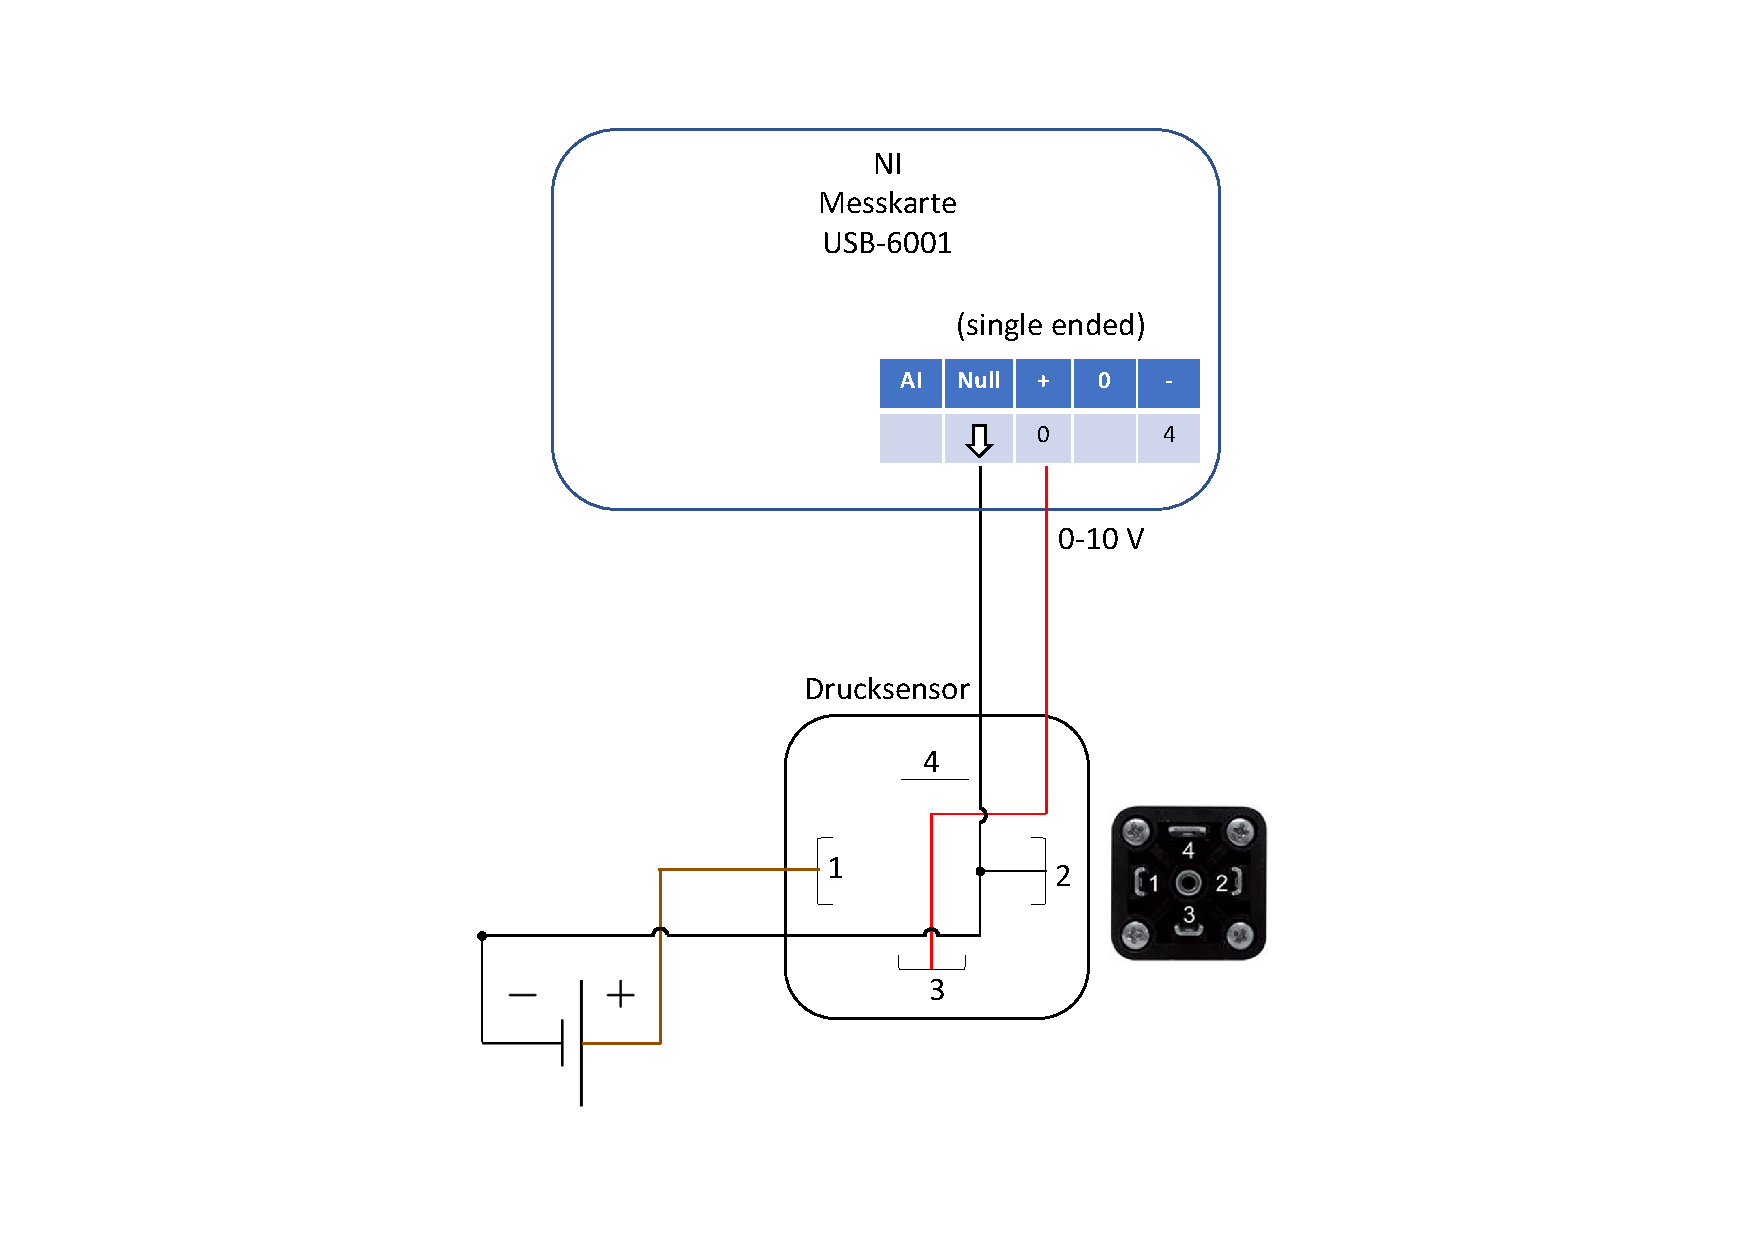
\includegraphics[width=1.02\textwidth]{Bilder/Filterkuchen_Messtechnik.pdf}
\vspace{-4em}
 \caption[]{Elektrotechnische Verschaltung der Komponenten der Filterkuchenversuchsanlage}\label{fig:filterkuchenelektrotechnik}
\end{figure}


Die Elektrotechnische Verschaltung des Drucksensors ist der Abbildung \ref{fig:filterkuchenelektrotechnik} zu entnehmen. Die Laborwaage des Typs Practum 5101-1S wird, via mitgelieferten USB-Y zu RS-232 Schnittstellenemulationsprozessorstecker Kabel, mit dem Desktop PC verbunden. 

\subsubsection{Filterkuchenversuchsanlage nach den Modifikationen}

In der Abbildung \ref{fig:filterkuchenversuchsstand_upgrade} ist die gesamte Filterkuchenversuchsanlage, nach dem Aufrüsten mit digitaler Sensorik zu erkennen. Die Grafik des Schlauchleitungs- und Gerätefließschemas ist der Abbildung  \ref{fig:schema_filterkuchenversuchsstand_upgrade} zu entnehmen. Der Versuchsaufbau wurde um eine Spannungsquelle ({\Hypatia N}) für den Drucksensor ({\Hypatia M}), einen Drucksensor ({\Hypatia M}), sowie ein Human-Machine-Interface (HMI, {\Hypatia O}) erweitert. Als HMI dient ein Desktop PC. Das Manometer zur Druckmessung bildet mit der Vacuumpumpe ({\Hypatia B}) eine Einheit. 

\subsubsection{Workflow der Filterkuchenversuchsanlagen}

In diesem Abschnitt wird der neue Workflow beschrieben. Die Datalogs werden derzeit in dem Datalogordner auf dem Desktop gespeichert. Der Tabelle \ref{tab:filterkuchenversuchsanlagenbezeichnungen} sind die Bezeichnungen der Komponenten zu entnehmen.

\begin{enumerate}
\item \textbf{{\Hypatia Starten des HMI}}
	\begin{itemize}
		\item Inbetriebnahme der Spannungsquelle
			\begin{enumerate}[label = \roman*]
			\item Hauptschalter auf der Rückseite betätigen
			\item Spannungshöhe zwischen 15 und 24 V einstellen
			\item On-button auf der Vorderseite betätigen $\Rightarrow$ Spannung stellt sich auf den gewählen Betrag ein
			\end{enumerate}	
	\item Waagensignalleitung ist mit der RS-232 Schnittstelle des HMI Towers zu verbinden.
	\item DAQ ist mit einem beliebigen USB Slot des HMI Towers zu verbinden
	\item Starten der LabVIEW Applikation \: {\Menlo Filterkuchenversuch\_V01DL.vi}
	\item Dateinamen eingeben: FK\_{\Menlo GruppenID.txt}
		\begin{enumerate}[label = -]
		\item Der Dateiname kann über den Versuchstag identisch bleiben, die Daten werden an das Datei\-ende angehängt.
		\end{enumerate}
	\item Tubidimeterdateinamen eingeben: FK\_Tubi\_{\Menlo GruppenID.txt}
		\begin{enumerate}[label = -]
		\item Der Dateiname kann über den Versuchstag identisch bleiben, die Daten werden pro Versuchsiteration überschrieben.
		\end{enumerate}
	\item Versuchseingaben tätigen
	\item wenn alle Vorbereitung der Filtrationseinrichtung \textbf{abgeschlossen} sind, dann
		\begin{enumerate}[label = \Roman*]
		\item Start des Programms: Das $\Rightarrow$ Icon oben links 
		\item öffnen des Absperrhahns H2
		\item wenn Messung abgeschlossen, dann
			\begin{enumerate}[label = --]
			\item Stop betätigen
				\begin{enumerate}[label = -]
				\item Filtratmenge bestimmen 
				\item Filterkuchendicke bestimmen 
				\item die trockene Filterkuchenmasse bestimmen
				\end{enumerate}
			\item Tubidimeter eingaben tätigen
			\item wenn abgeschlossen,  starten der nächsten Iteration bei I		 
			 \end{enumerate}
			\item \textbf{Nach der letzten Tubidimetereingabe ist das Programm nochmals zu starten und der Stop-button zu betätigen, damit die aktuellsten Tubidimeterdaten in der \newline FK\_Tubi\_{\Menlo GruppenID.txt} gespeichert werden!} 
		\end{enumerate}	
	\end{itemize}


\item \textbf{{\Hypatia Vorbereitung der Filtrationseinrichtung}}
	\begin{enumerate}[label = \alph*]
	\item Absperrhahn H1 schließen
	\item Filtrationsanlage evakuieren, dazu ist die \textit{manuell} Taste des Vakuumcontrollers zu betätigen. Bei erreichen des Solldrucks wird der isobare Zustand der Anlage erhalten.
 	\item Gereinigte Filternutsche ({\Hypatia I}) in der Kunststoffklemmvorrichtung ({\Hypatia G}) fixieren.
 	\item Es ist darauf zu achten, dass der Metallsteg der Nutschenhalterung nach vorn zeigt
	\item Absperrhahn H2 schließen (Hebelstellung: waagerecht).
	\item Schläuche sachgemäß montieren.
	\item Schutzplatte der Waage entfernen und daraufhin einschalten.	
	\item Einfüllen der Suspension und Inbetriebnahme des Rührers. 
	\item Öffnen des Dreiwegehahns H1
	\item Wenn alle Vorbereitungen abgeschlossen sind und die angezeigte Masse Konstant ist, ist die Waage zu tarieren.
	 \end{enumerate}	
\end{enumerate}

 

\begin{figure}[p!] % 
% \captionsetup{position=top}
    \centering
        \subfloat[][Filterkuchenversuchsanlage nach den Modifikationen \label{fig:filterkuchenversuchsstand_upgrade}]{%
            \hspace{0em}
            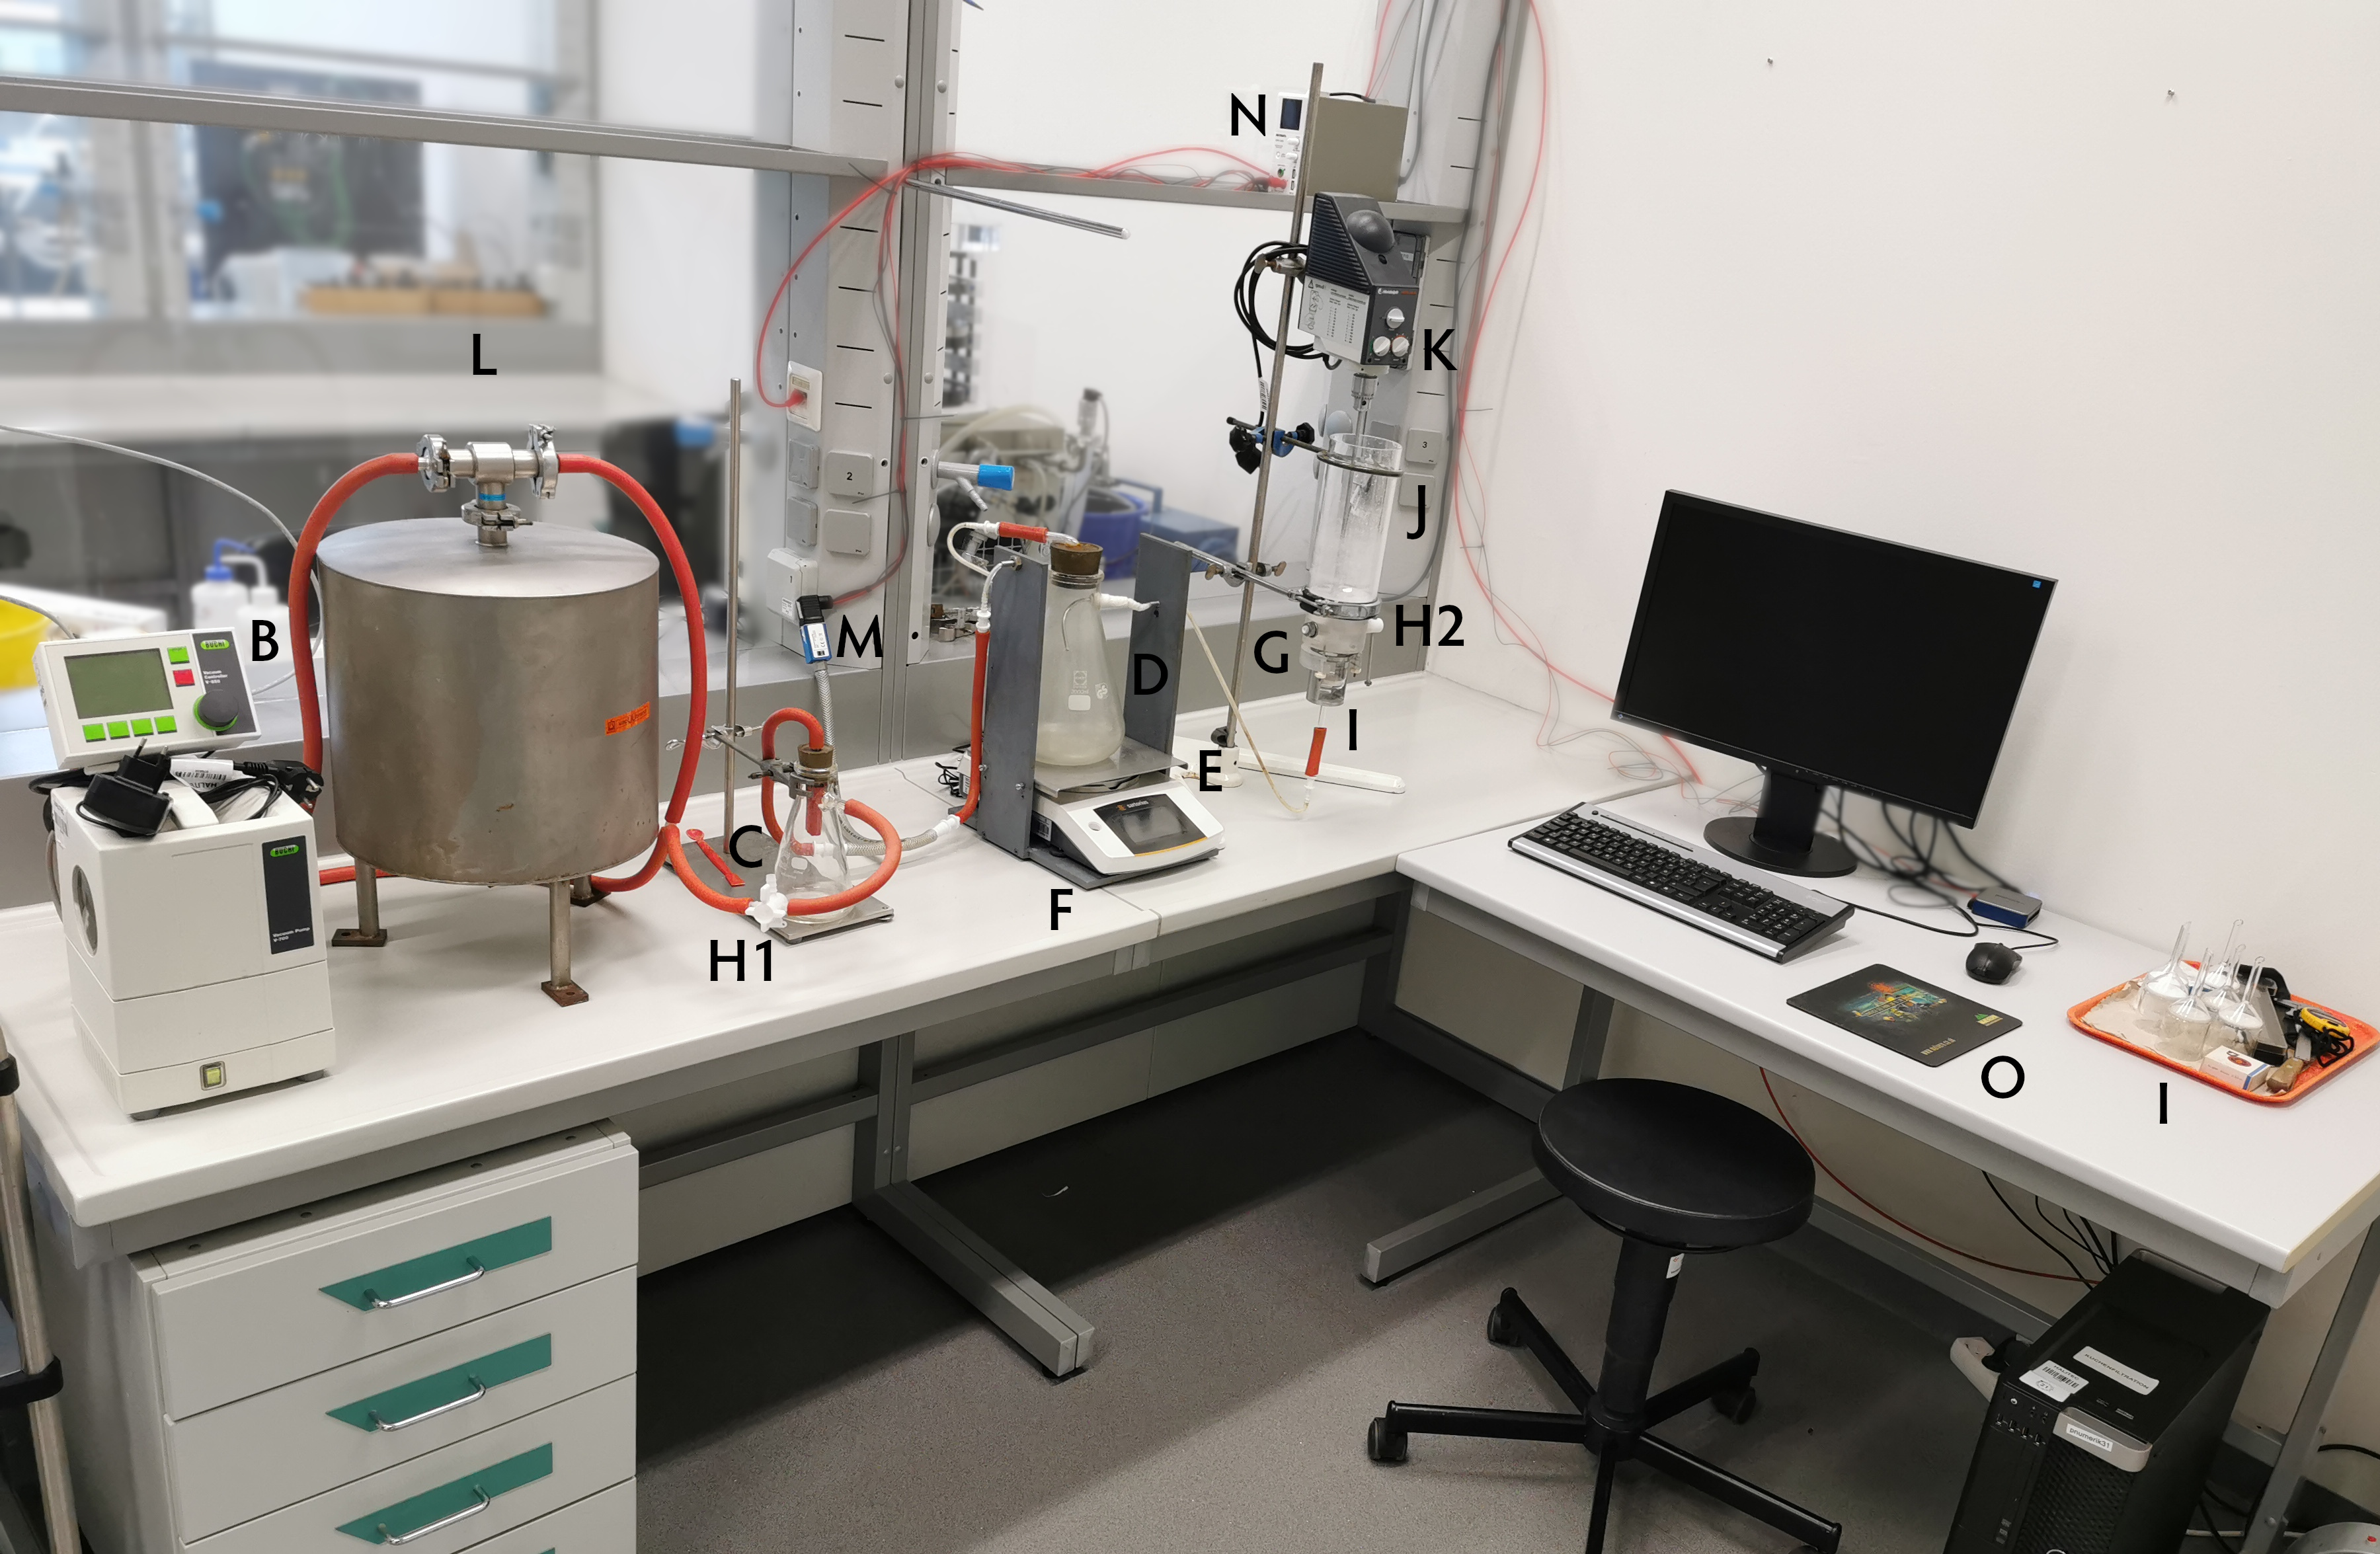
\includegraphics[width=1\textwidth]
            {Bilder/HAW/filterkuchenversuchsanlage_upgrade.jpg} %{Bilder/LabVIEW_serialport/}
        }
    \phantomcaption
    \vspace{1em}
    \ContinuedFloat
%\captionsetup{position=bottom}
    \subfloat[Fließschema in Form einer schematischen Skizze der Filterkuchenversuchsanlage nach den Modifikationen][Fließschema in Form einer schematischen Skizze der Filterkuchenversuchsanlage nach den Modifikationen \cite{Kuchenfiltration_Geweke2020} \label{fig:schema_filterkuchenversuchsstand_upgrade}]{%
        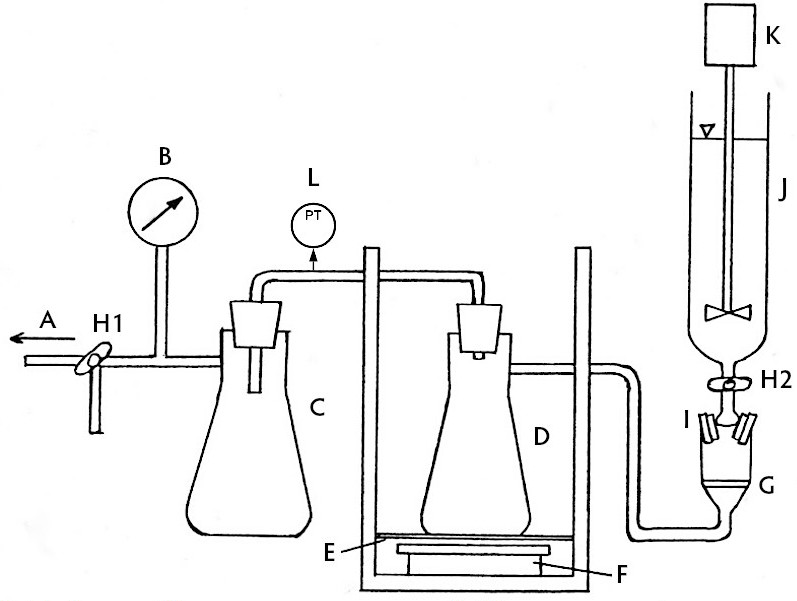
\includegraphics[width=0.65\textwidth]
        {Bilder/filterkuchversuch_schema_upgrade.jpg} %{Bilder/LabVIEW_serialport/}
    }
    \caption[]{Filterkuchenversuchsanlage nach dem Aufrüsten mit digitaler Sensorik }
    \label{fig:Filterkuchenversuchsanlage_bezeichnet_upgrade}
\end{figure}

\begin{table}[h!]
\centering
\caption{Bezeichnungen der Filterkuchenversuchsanlage}\label{tab:filterkuchenversuchsanlagenbezeichnungen}
\vspace{0.5em}
{\Hypatia \begin{tabular}{r l r l}
A & Verbindung zur Vacuumpumpe 				&  H2	& Absperrhahn	\\[0.1em]
B 	& Vacuummanometer 								& I	& Filternutsche 		\\[0.1em]  
C & Rezipient und Wasserabscheider \quad \quad	& J & Trübebehälter  \\[0.1em]
D	& Filtratauffangbehälter    							& K 	& Rührer 				\\[0.1em]	
E & Schutzplatte für Waage 							&  L & Pufferbehälter		\\[0.1em]
F 	& Waage mit digitaler Schnittstlelle 				& M & Drucksensor 		\\[0.1em]	
G & Kunststoffklemmvorrichtung									& N & Spannungsquelle \\[0.1em]	
 & --~\,Gummidichtung 									& O & HMI (Human-Machine-Interface)\\[0.1em]	
H1 &  	Dreiwegehahn									& 		& \\ 
\end{tabular}}
\end{table}



\newpage
\subsection{Wirbelschichtversuchsanlage}

Das verfahrenstechnische Labor der HAW-Hamburg Life Sciences besitzt eine Wirbelschichtversuchsanlage im Labormaßstab (siehe Abbildung \ref{fig:Wirbelschicht_mod0}). In der Abbildung \ref{fig:Wirbelschicht_konzept} ist eine Versuchsskizze des Versuchsstands dargestellt. Der gesamten Anlage ist ein Druckminderer vorgeschaltet ({\Hypatia A}). Um den Volumenstrom zu Steuern, befindet sich nach dem Druckminderer ein Handventil ({\Hypatia B}). Zur Detektion des Volumenstroms sind zwei Schwebekörperdurchflussmesser (SKDM) ({\Hypatia C}) in reihe nachgeschaltet, um einen Volumenstrom von bis zu 50~l/min Messen zu können. Mit dem SKDM auf der rechten Seite kann der Messbereich von von 0,185~bis~5~l/min gemessen werden. Mit dem SKDM auf der linken Seite sind Volumenströme 1,86~bis~50~l/min messbar. Vor dem Anströmboden muss ein Druck gemessen werden, dafür befindet sich am Boden des Fluidisierapparats ({\Hypatia E}) ein kleiner Flansch, mit dem der Druck relativ zur Umgebung mittels U-Rohr Manometer ({\Hypatia D}) gemessen werden kann. Der Fluidisierapparat besteht aus einer Plexiglassäule und dem Boden, in dem ein Gewebefilter eingespannt ist. Da Partikel mit dem Volumenstrom ausgetragen werden können, befindet sich über dem Fluidisierapparat eine Absaugung ({\Hypatia F}).

Bei diesem Versuch sind im Verlauf der Versuchsdurchführung die folgenden Parameter zu erfassen:

\begin{enumerate}[label = \textbullet, itemsep = -.1em]
\item \textbf{diskret}
	\begin{enumerate}[label = --, itemsep = -.1em]
		\item Festbettbetthöhe $h_{\mathrm{fb}}$
		\item Festbettporösität $\varepsilon_{\mathrm{fb}}$
		\item Schüttgutmasse $m_{\mathrm{Schüttgut}}$
		\item Partikeldichte $\rho_{\mathrm{fs}}$
		\item Sauterdurchmesser
	\end{enumerate}  	
	
\item \textbf{kontinuierlich}
	\begin{enumerate}[label = --, itemsep = -.1em]
		\item $\dot{V}_{\mathrm{Luft}}$ 
		\item $\Delta p (t)$ 
	\end{enumerate} 
	
\item \textbf{kontinuierlich/diskret}
	\begin{enumerate}[label = --, itemsep = -.1em]
		\item Wirbelschichthöhe $h_{\mathrm{ws}} = f(p)$
		\item Wirbelschichtporösität $\varepsilon_{\mathrm{ws}}= f(p)$ 
	\end{enumerate} 
	
\end{enumerate} 

\begin{figure}[p!] % Wirbelschichtversuchsanlage der HAW Hamburg der Fakultät Life Sciences
%\captionsetup{position=top}
\centering
     \subfloat[]
     [Wirbelschichtversuchsanlage vor den Modifikationen \label{fig:Wirbelschicht_mod0}]{%
       \hspace{0em}
       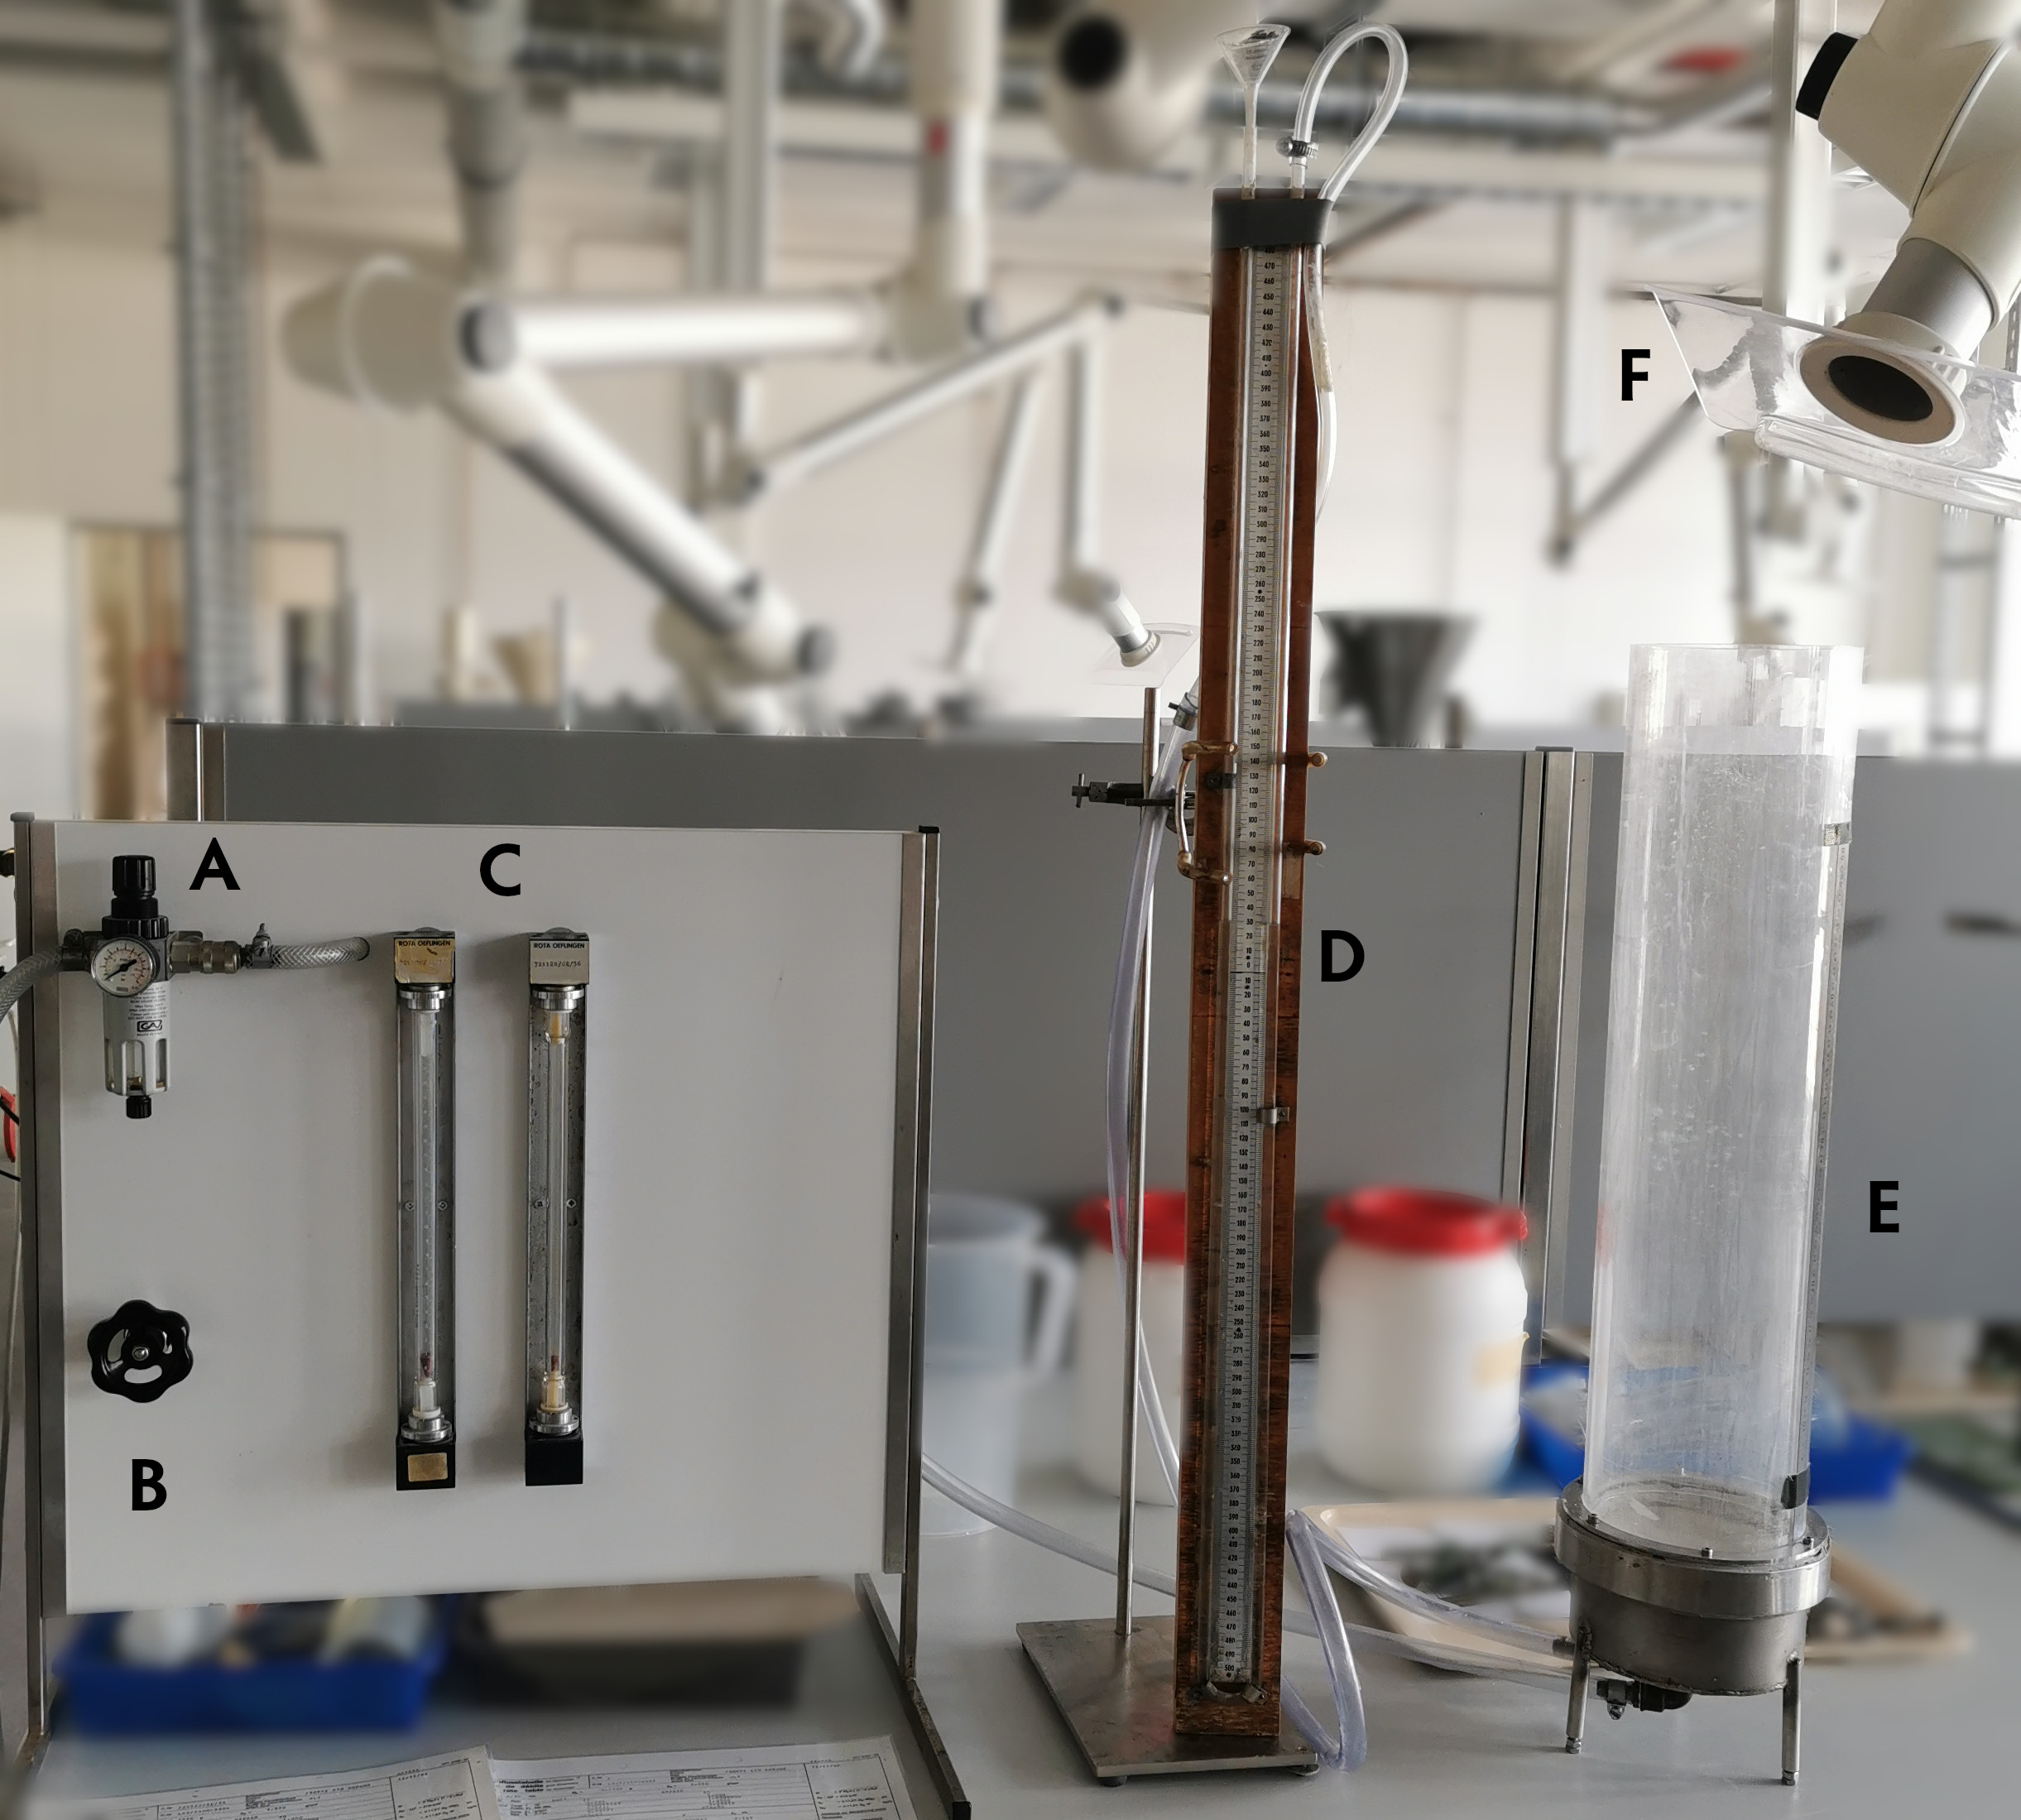
\includegraphics[width=0.8\textwidth]
       {Bilder/HAW/Wirbelschicht.jpg} %{Bilder/LabVIEW_serialport/}
     }
\phantomcaption
\vspace{1em}
\ContinuedFloat
%\captionsetup{position=bottom}
	\subfloat[][Schematische Skizze des Wirbelschichtversuchs vor den Modifikationen \label{fig:Wirbelschicht_konzept}]{%
    	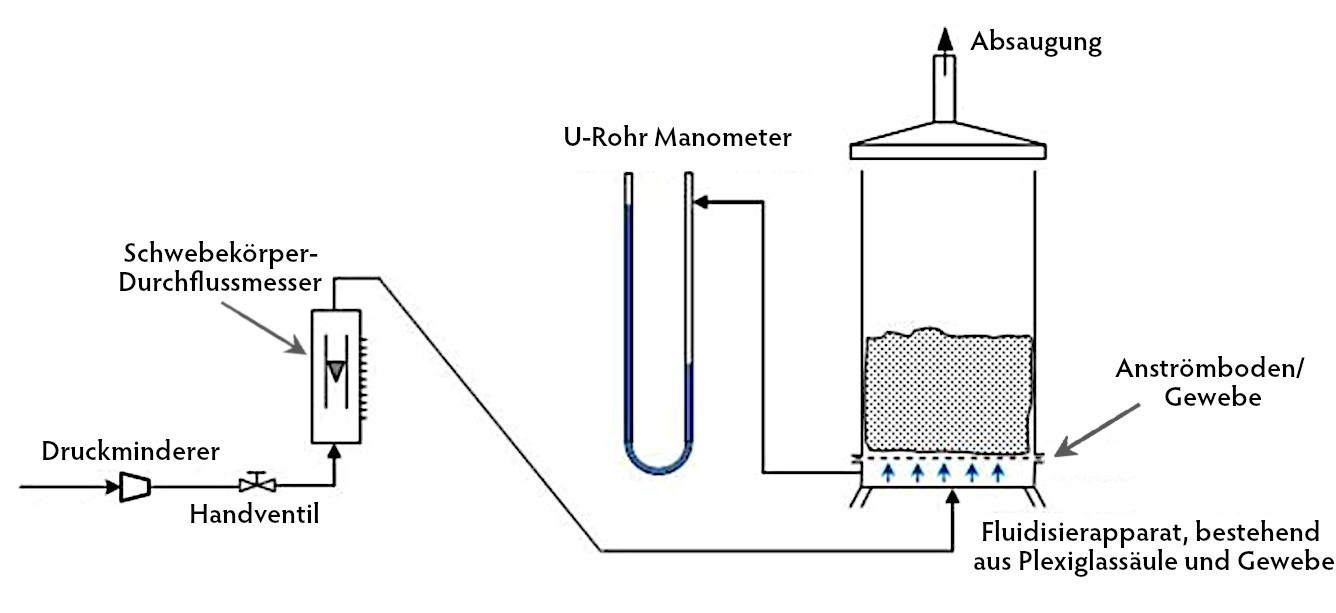
\includegraphics[width=1\textwidth]
        {Bilder/HAW/Wirbelschicht_konzept.jpg} %{Bilder/LabVIEW_serialport/}
       	}
\caption[Wirbelschichtversuchsanlage der HAW Hamburg der Fakultät Life Sciences, vor den Modifiktationen]{Wirbelschichtversuchsanlage der HAW Hamburg der Fakultät Life Sciences, vor den Modifiktationen}
\label{fig:Wirbelschicht}
\end{figure}


\newpage




Es ist hinreichend, die Wirbelschichthöhe und die daraus resultierende Porösität diskret zu erfassen. Im Rahmen dieser Arbeit wird die diskrete, manuelle Erfassung gewählt. Im Anhang befindet sich ein Diagramme für den SKDM der Messspanne von 0,185~bis~5~l/min (Abbildung \ref{fig:kleiner_skdm}) und ein Diagramm für den SKDM der Messspanne von 1,86~bis~50~l/min (siehe Abbildung \ref{fig:grosser_skdm}). Beide Diagramme enthalten Kennlinien der SKDM zzgl. jeweils zwei Approximationsfunktionen. Des Weiteren befindet sich eine Manometerkennlinie, siehe Abbildung \ref{fig:manometer_kennlinie}.\\


\subsubsection{Sensorauswahl}

Im Betrieb der Anlage sind die kontinuierlichen Parameter Volumenstrom $\dot{V}$ und Druck $p$ messtechnisch zu erfassen. Die zu erfassenen Druckdifferenzen bei diesem Versuchsstand sind ebenfalls gering, daher wird ein piezoresistiver Relativdrucksensor des Unternehmens B+B Thermo-Technik GmbH des Typs DRTR-AL-10V-RV1 gewählt. Die Messspanne dieses Sensors ist von -1~-~1~bar. Die Spanne des analogen Ausgangssignals ist von 0~-~10~V. Die Technischen Daten sind der Tabelle \ref{fig:BTTG2021} im Anhang zu entnehmen. \\

Gemäß Abschnitt \ref{sec:digi_durchfluss} sind diverse Durchflussensoren geeignet, um den Luftvolumenstrom zu erfassen. Differenzdrucksensoren sind für kleine Messbereiche nicht geeignet. Gemäß der Randbedingung des Versuchs, sind die folgenden Drucksensoren potentiell möglich.

\begin{itemize}
\item Vortexsensor
\item Drallsensor
\item Coriolissenor
\item thermischer Massendurchflussensor
\end{itemize}  

Da vor einer Kostenanalyse der Sensoren eine Anschaffung eines thermischen Massendurchflussensor des Typs VA-525 des Unternehmens CS Instruments GmbH \& Co. KG mit einer Messspanne von 0,02~-~50~l/min erfolgt ist, wird ein Vergleich der Randbedingungen und des finanziellen Aufwands im Rahmen dieser Arbeit nicht erfolgen. Das Kalibrierzertifikat des Durchflusssensors ist dem Anhang zu entnehmen (siehe Abbildung \ref{fig:va-525_kalib}). \newpage


\subsubsection{Elektrotechnik der Wirbelschichtversuchsanlage}
\label{sec:schaltung}
Die Sensorik ist elektrotechnisch zu verschalten, die genutzten Komponenten sind:

\begin{itemize}
\item als Spannungsquelle ein Transformator des Typs Voltcraft TOPS-3205   
\begin{itemize}
\item Conrad Electronic AG
\end{itemize}

\item ein Strom- Spannungswandler des Typs WAA 7-0541 
\begin{itemize}
\item Friedrich Lütze GmbH \& Co. KG
\end{itemize}

\item ein Drucksensor des Typs DRTR-AL-10V-RV1
\begin{itemize}
\item B+B Thermo-Technik GmbH
\end{itemize}

\item ein thermischer Massendurchflusssensor des Typs VA-525
\begin{itemize}
\item CS Instruments GmbH \& Co. KG
\end{itemize}

\item eine DAQ Messkarte (\textit{engl. data acquisition}) des Typs USB-6001 
\begin{itemize}
\item National Instruments (NI)
\end{itemize}
\end{itemize}

In der Abbildung \ref{fig:wirbelelektrotechnik} ist ein Schema der elektrotechnischen Verschaltung dargestellt. Der Volumenstromsensor generiert analoge Messwertsignale der Spanne 4~bis~20~mA. Die DAQ Messkarte kann analoge  Signale der Spanne 0~bis~10~V in ein digitales Signal umwandeln, daher ist zwischen dem Durchflussensor und dem DAQ ein Strom- Spannungswandler zu implementieren. Der Stromspannungswandler benötigt eine Spannungsquelle (Klemmen 1 und \textcolor{brown}{6}). Die analogen Signale des Volumenstromsensors (\textcolor{brown}{1}) und (3) werden am Stromspannungswandler an (2) und (\textcolor{black!50}{3}) angeklemmt. Die umgewandelten Signale treten aus den Klemmen (\textcolor{red}{4}) und (5) des Wandler aus. \textbf{Dieses Signal ist an einem DAQ nun differenziell zu verschalten}. Das \,{\Menlo minus} (-) Signal wird an der Messkarte demnach nicht über \,{\Menlo Null} (\textit{engl. Ground}), sondern an \,{\Menlo minus} angeklemmt. \\

Der Drucksensor generiert analoge Messsignale der Spanne 0~bis~10~V. Die Ausgänge des Sensors (2) und (\textcolor{red}{3}) sind mit \,{\Menlo Null} und \,{\Menlo plus} (+) zu verschalten. Es ist anzumerken, dass die Slots im DAQ willkürlich so gewählt wurden. Sollten die Slots gewechselt werden, dann muss es im Blockdiagramm des Hauptprogramms angepasst werden.\\


\begin{figure}[t!] %[htbp!] 
\centering
\vspace{-7em}
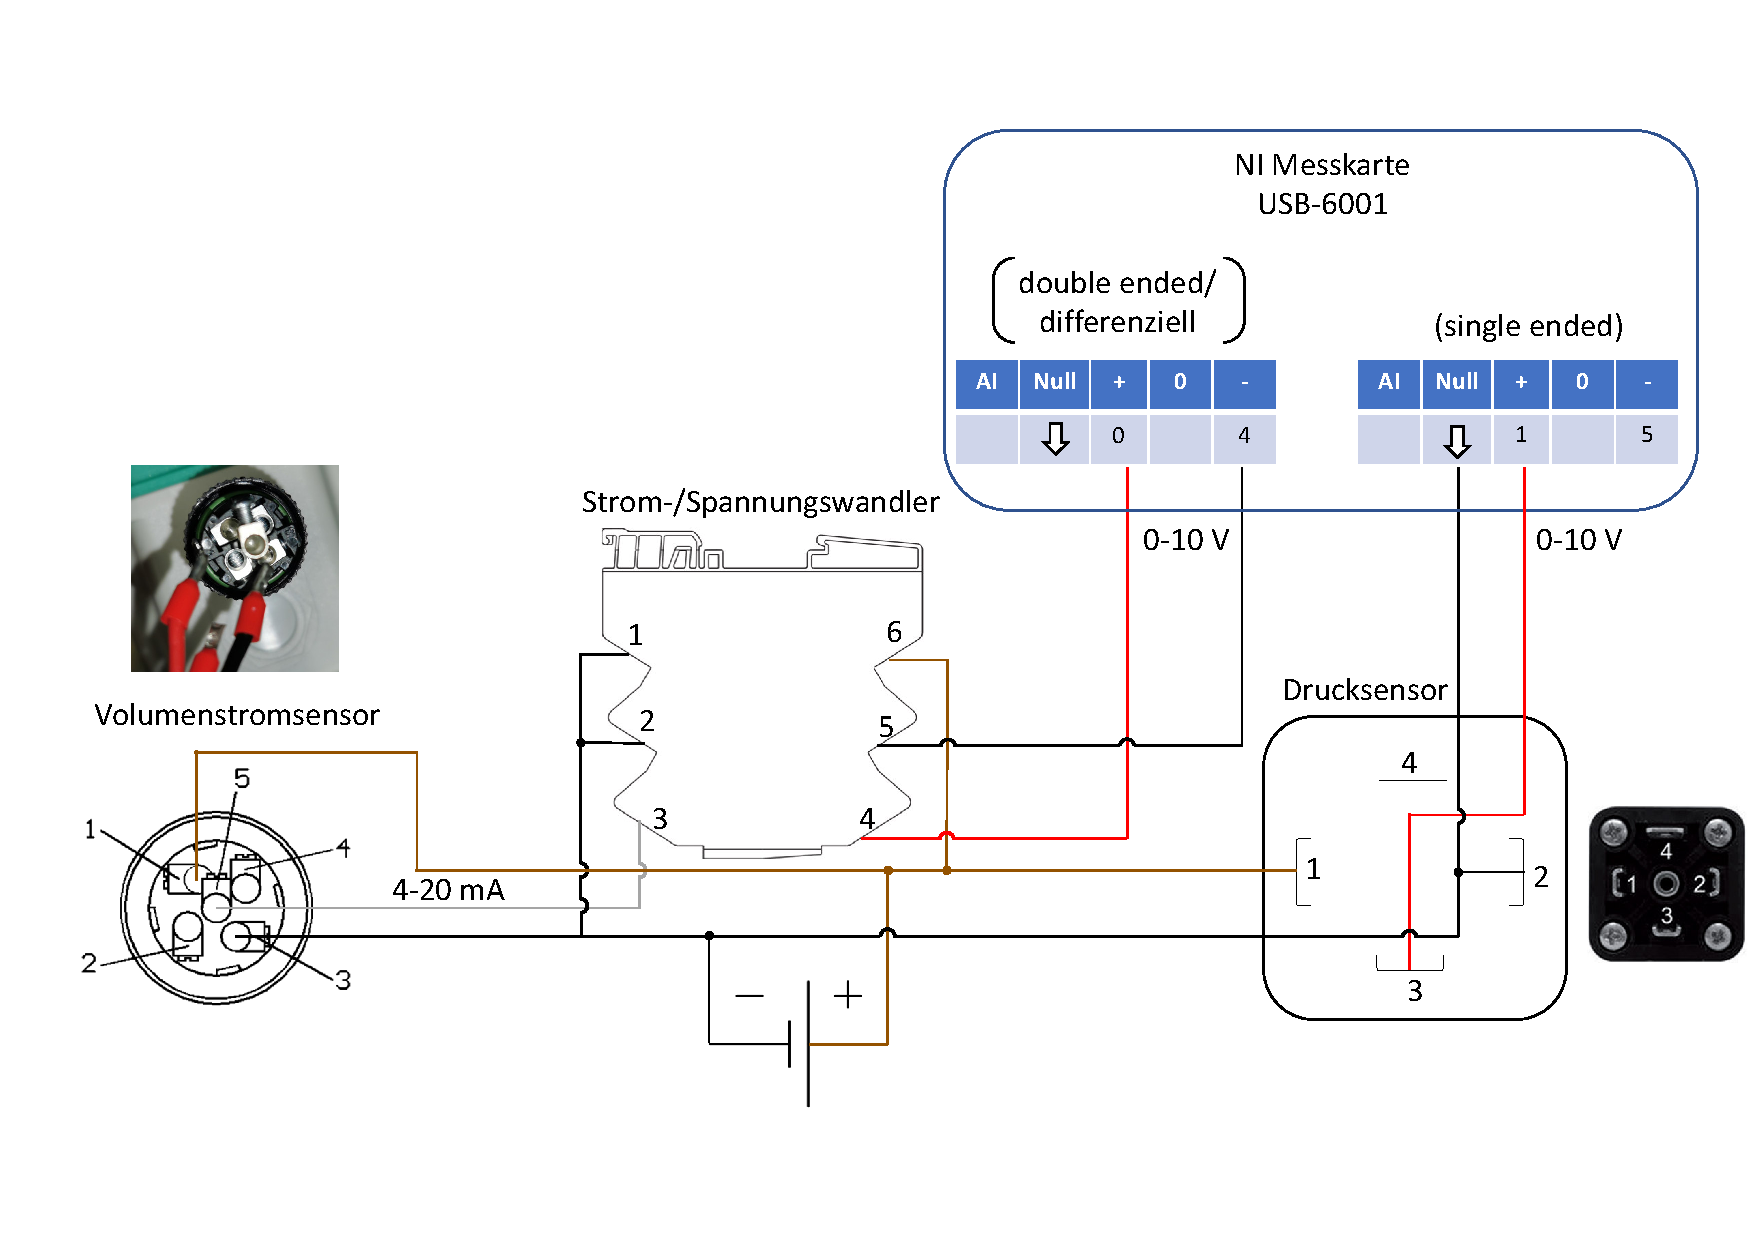
\includegraphics[width=1.02\textwidth]{Bilder/Wirbelschicht_Messtechnik.pdf}
\vspace{-4.5em}
 \caption[]{Elektrotechnische Verschaltung der Komponenten der Wirbelschichtversuchsanlage}\label{fig:wirbelelektrotechnik}
\end{figure}

\subsubsection{Wirbelschichtversuchsanlage nach den Modifikationen}

In der Abbildung \ref{fig:Wirbelschicht_upgrade} ist die Wirbelschichtversuchsanlage nach der Implementation des Druck und Volumenstromsensors zu erkennen. In der Abbildung \ref{fig:Wirbelschicht_konzept_modifiziert} ist das Fließschema der aufgerüsteten Wirbelschichtversuchsanlage abgebildet. Der Tabelle \ref{tab:bezeichnungstabelle_nach_den Modifikationen} sind die Bezeichnungen der Komponenten, der Wirbelschichtanalge nach den Modifikationen, zu entnehmen. Dem Druckminderer ({\Hypatia A}) ist das Handventil ({\Hypatia B}), zur manuellen Volumenstromsteuerung, nachgeschaltet. Nach den SKDM ({\Hypatia C}) ist der Volumenstromsensor ({\Hypatia D}) des Typs VA-525 nachgeschaltet. Nach dem Volumenstromsensor wurde ein Drucksensor ({\Hypatia E}) des Typs DRTR-AL-10V-RV1, wie auch der Volumenstromsensor, als diversitäre Redundanz implementiert. Der Drucksensor, wie auch das Manometer ({\Hypatia F}), misst den Druck vor dem Anströmboden. Über dem Fluidisertopf ({\Hypatia H}) ist eine Absaugung ({\Hypatia I}) positioniert. Wie der Abbildung  \ref{fig:Wirbelschicht_upgrade} zu entnehmen, ist es möglich eine weitere Absaugung  über dem HMI ({\Hypatia L}) zu positionieren. Des Weiteren sind weitere messtechnische Komponenten hinzugekommen. Als DAQ Messkarte wird ein Gerät des Unternehmens National Instruments des Typs USB-6001 ({\Hypatia K}) verwendet. Der Strom-/Spannungswandler ({\Hypatia G}) ist an der Trennwand befestigt. Als Spannungsversorgung für den Volumenstromsensor ({\Hypatia D}), dem Drucksensor ({\Hypatia E}), dem Strom-/Spannungswandler ({\Hypatia G}) und dem DAQ ({\Hypatia K}), wird ein Transformator ({\Hypatia \,J}) des Typs TOPS-3205 von Voltcraft verwendet.\\



\begin{table}[h!]
\caption{Bezeichnungen der Wirbelschichtversuchsanlage nach den Modifikationen} \label{tab:bezeichnungstabelle_nach_den Modifikationen}
\begin{center}
{\Hypatia \begin{tabular}{rl r l}
A & Druckminderer 						& H & Fluidisiertopf  \\[0.1em]
B & Handventil 	 							& &  --~\, Plexiglassäule\\[0.1em]
C & Schwebekörperdurchflussmesser \quad \quad 		& & -- ~\,Gewebefilter als Anströmboden  \\[0.1em]
D & thermischer Durchflusssensor 	&  I & Absaugungen \\[0.1em]
E & piezoresistiver Drucksensor	 	& J & Spannungsquelle \\[0.1em]
F & U-Rohr Manometer 					&	K & NI DAQ USB-6001 \\[0.1em]
G & Strom-/Spannungswandler	 	&  L  & HMI (Human-Machine-Interface)\\[0.1em]				
\end{tabular}}
\end{center}
\end{table}

\begin{figure}[t!] % Wirbelschichtversuchsanlage nach den Modifikationen
% \captionsetup{position=top}
    \centering
        \subfloat[Wirbelschichtversuchsanlage nach den Modifikationen]
        [Wirbelschichtversuchsanlage nach den Modifikationen \label{fig:Wirbelschicht_upgrade}]{%
            \hspace{0em}
            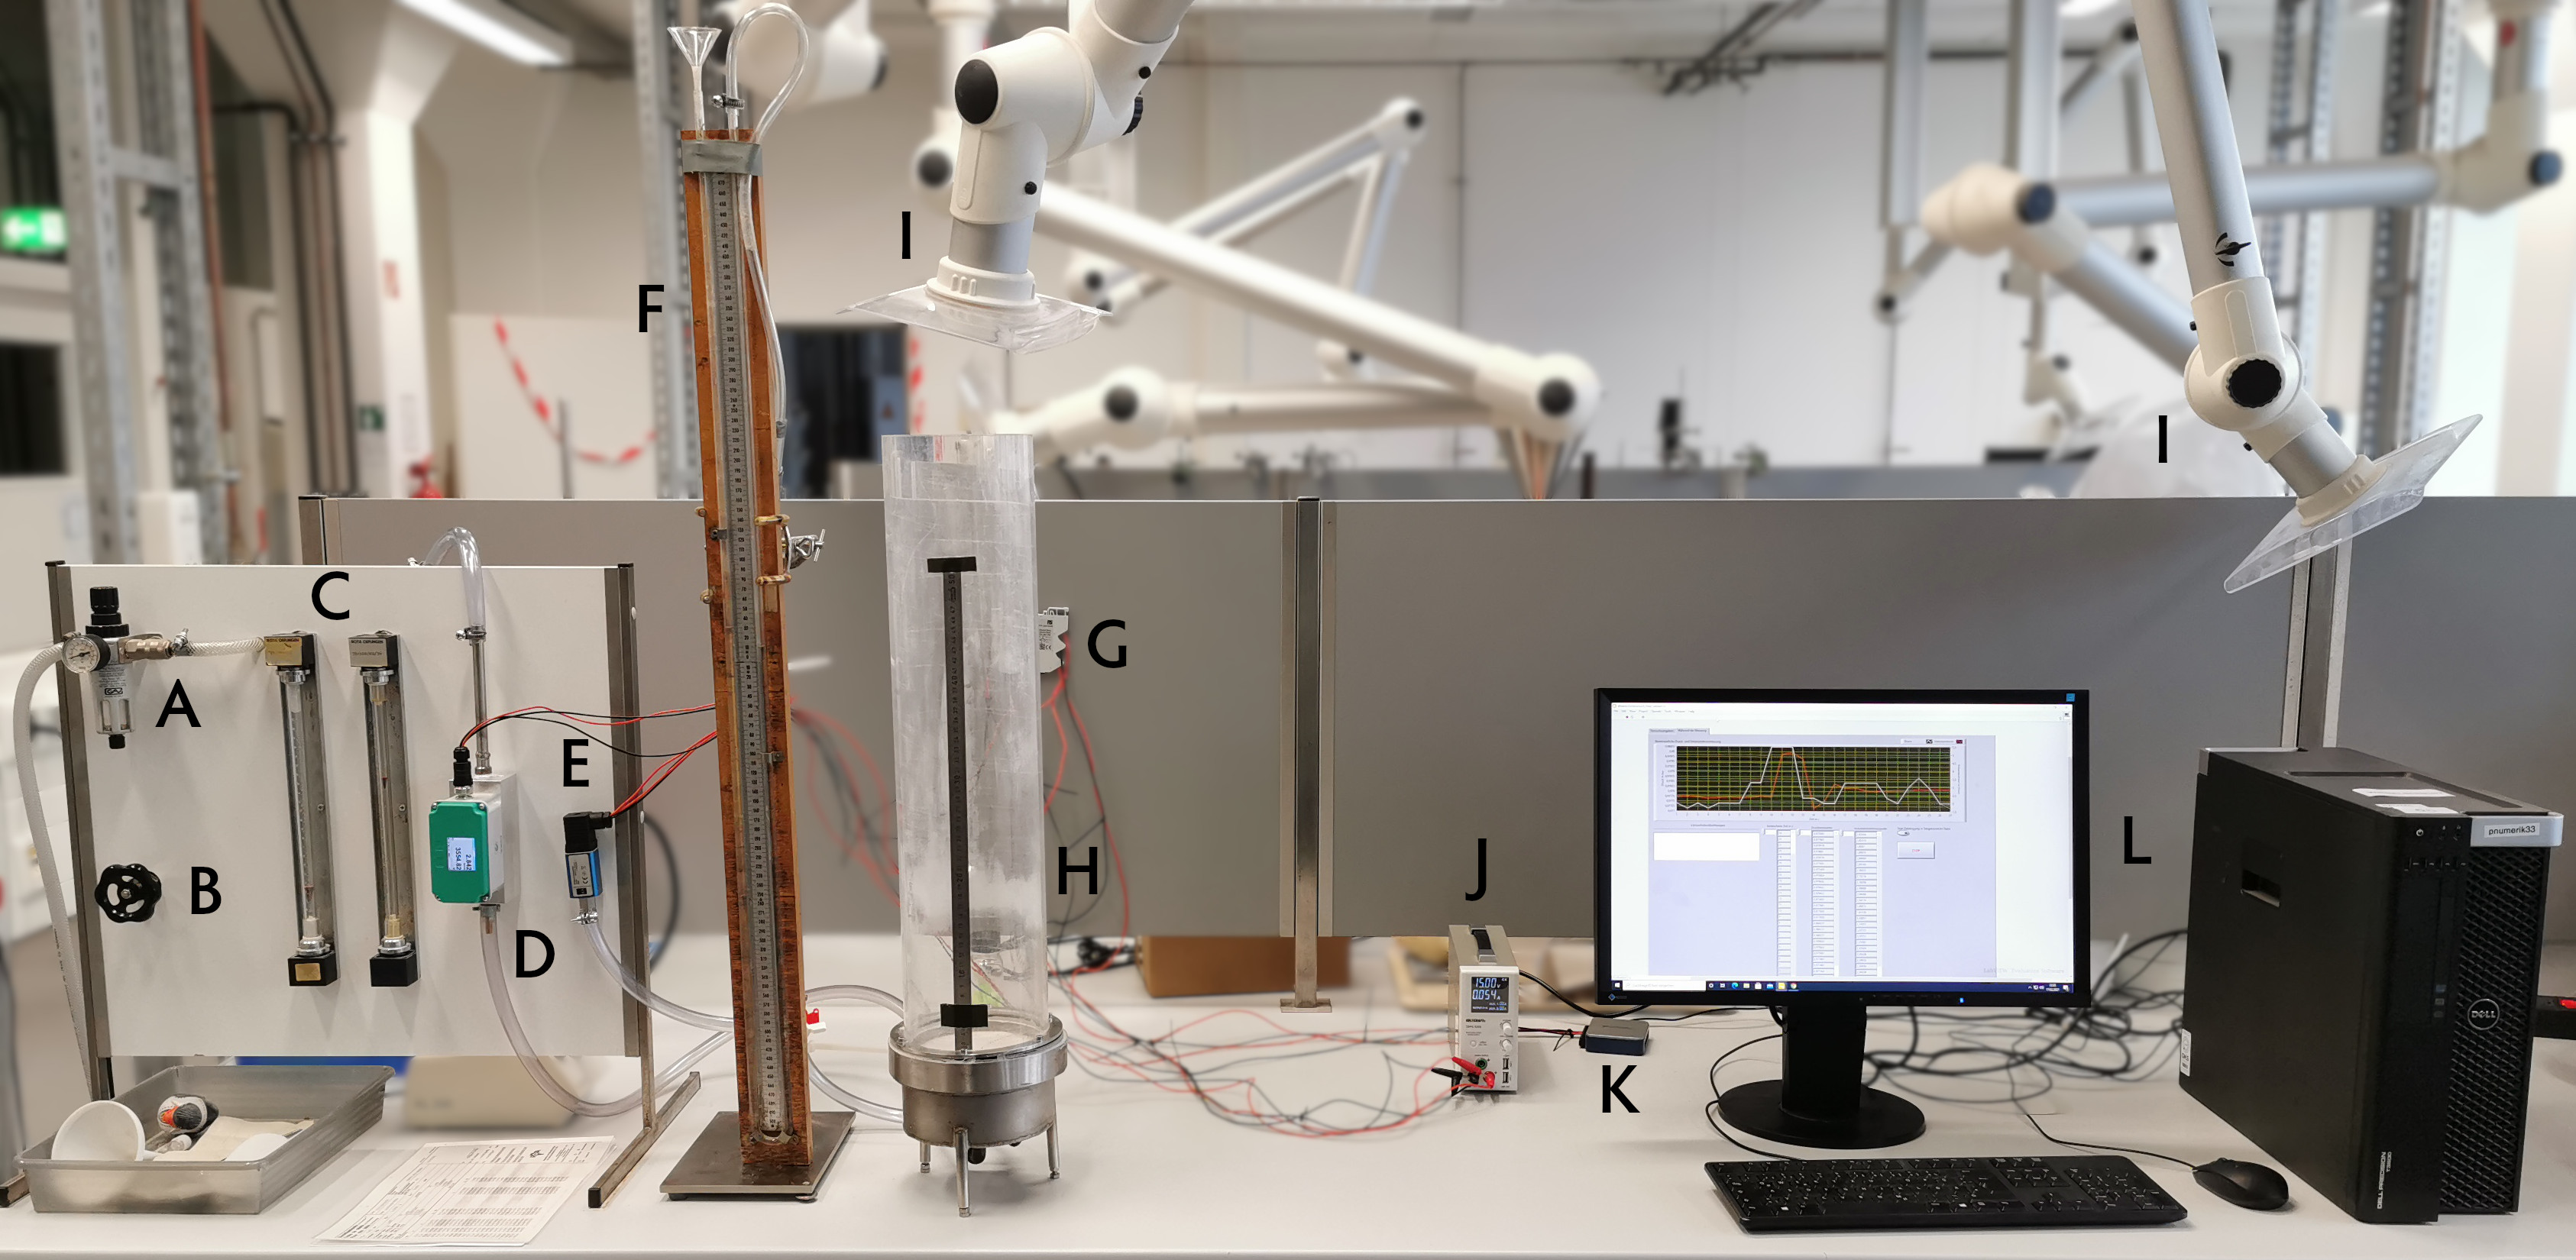
\includegraphics[width=1.05\textwidth]
            {Bilder/HAW/Wirbelschicht_upgrade.jpg} %{Bilder/LabVIEW_serialport/}
        }
    \phantomcaption
    \vspace{1em}
    \ContinuedFloat
% \captionsetup{position=bottom}
    \subfloat[][Fließschema in Form einer schematischen Skizze der Wirbelschichtversuchsanlage nach den Modifikationen \label{fig:Wirbelschicht_konzept_modifiziert}]{%
        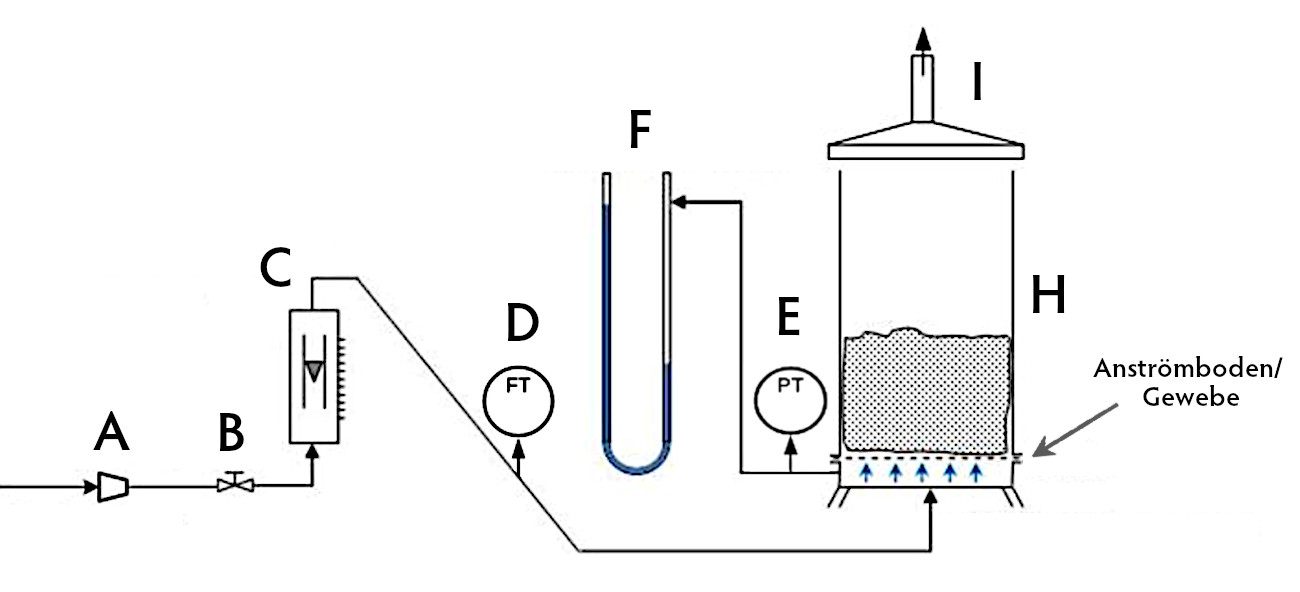
\includegraphics[width=0.8\textwidth]
        {Bilder/HAW/Wirbelschicht_konzept_modifiziert.jpg} %{Bilder/LabVIEW_serialport/}
    }
    \caption[]{Wirbelschichtversuchsanlage nach dem Aufrüsten mit digitaler Sensorik}
    \label{}
\end{figure}


\subsubsection{Workflow der Wirbelschichtanlage}

In diesem Abschnitt wird der neue Workflow der Wirbelschichtanlage beschrieben. Die Datalog-Datei wird derzeit ebenfalls in dem Datalogordner auf dem Desktop gespeichert.

\begin{enumerate}
\item \textbf{{\Hypatia Starten des HMI}}
	\begin{enumerate}[label = \Roman*, itemsep = -.1em]
		\item Inbetriebnahme der Spannungsquelle
			\begin{enumerate}[label = \roman*, itemsep = -.1em]
			\item Hauptschalter auf der Rückseite betätigen
			\item Spannungshöhe zwischen 15 und 24 V einstellen
			\item On-button auf der Vorderseite betätigen $\Rightarrow$ Spannung stellt sich auf den gewählen Betrag ein
			\end{enumerate}	
			
	\item DAQ ist mit einem beliebigen USB Slot des HMI Towers zu verbinden.
	\item Starten der LabVIEW Applikation {\Menlo Wirbelschichtversuch\_V01DL.vi}
	\item Datalognamen eingeben: WS\_{\Menlo GruppenID.txt}
	
		\begin{enumerate}[label = -, itemsep = -.1em]
		\item Der Dateiname kann über den Versuchstag identisch bleiben, die Daten werden an das Dateiende angehängt
		\end{enumerate}
	\item Versuchseingaben tätigen
	\item Start des Programms: Das $\Rightarrow$ Icon oben links 
	
\end{enumerate}
\item \textbf{{\Hypatia Praktische Versuchsdurchführung }}
\begin{itemize}
\item Druckleitung öffnen
\item Handventil zur manuellen Steuerung des Volumenstroms nutzen
\end{itemize}
\end{enumerate}

\subsubsection{Fazit}

Der Versuchsstand wurde mit geeigneter Sensorik aufgerüstet, um die kontinuierlichen Parameter, Druck $p$ und Volumenstrom $\dot{V}$, zu erfassen. Die Signale des Drucksensors sind von 0~bis~10~V und die des thermischen Massendurchflusssensors sind von 4~bis~20~mA. Eine digitale Erfassung der Festbett- bzw. Wirbelschichthöhe ist denkbar. Bei bedarf könnten bspw. geeignete optische, akustische, mechanische Entfernungsmesser, im Rahmen einer studentischen Projektarbeit, recherchiert und umgesetzt werden. Des Weiteren könnte die Steuerung des Volumenstroms, derzeit per Handventil, durch eine digitale Steuerung ersetzt werden. Der derzeitige Volumenstromsensor (VA-525) könnte entfernt und für andere Versuchsaufbauten verwendet werden.
\pagebreak

